\documentclass[11pt]{article}
\usepackage[margin=1in]{geometry}
\usepackage{amsmath, amssymb, amsthm, esint, physics}
\usepackage{fancyhdr}
\usepackage{tikz, tikz-3dplot}
% \usepackage{hyperref}
\usepackage{enumitem}
\usepackage{caption}
\usepackage{float}

% Page setup
\pagestyle{fancy}
\setlength{\headheight}{14pt}
\fancyhf{}
\lhead{Single Variable Calculus: Integral}
\cfoot{\thepage}

\begin{document}
\pagestyle{plain}
\begin{center}
  \tableofcontents
\end{center}
\newpage
\setcounter{page}{1}
\pagestyle{fancy}

\section{Antiderivatives and Indefinite Integrals}
\subsection{Definition}
A function $F(x)$ is called an \textbf{antiderivative} of a function $f(x)$ on an interval $I$ if
\[
    F'(x) = f(x) \quad \text{for all } x \in I.
\]The set of antiderivatives of $f$ is called the indefinite integral of $f$.\\[.5em]
\textbf{Notation:}
The indefinite integral of $f(x)$ is denoted by
\[
    \int f(x)\,dx = F(x) + C,
\]
where $C$ is an arbitrary constant called the \textbf{constant of integration}.
\subsection{Property of Indefinite Integrals}
$
  \begin{array}{l}
    \displaystyle
    \qquad\int f(x)\,dx = F(x)+C \iff F'(x) = f(x)\\[10pt]
    \displaystyle
    \qquad\int af(x)\,dx = a\int f(x)\,dx\\[10pt]
    \displaystyle
    \qquad\int [f(x)\pm g(x)]\,dx = \int f(x)\,dx \pm \int g(x)\, dx
  \end{array}
$
\section{Integration Formulas}
\subsection{Polynomials}
$
  \begin{array}{l}
    \displaystyle
    \qquad\int \,dx = x + C\\[10pt]
    \displaystyle
    \qquad\int a\,dx = ax + C\\[10pt]
    \displaystyle
    \qquad\int x^n\,dx = \frac{x^{n+1}}{n+1}+C\quad, n\neq-1
  \end{array}
$
\subsection{Exponential and Logarithmic Functions}
$
  \begin{array}{l}
  \qquad\displaystyle \int  e^x\,dx = e^x+C\\[10pt]
  \qquad\displaystyle \int \frac{1}{x}\,dx= \ln|x|+C\\[10pt]
  \qquad\displaystyle \int a^x\,dx = \frac{a^x}{\ln a}+C
  \end{array}
$
\subsection{Trigonometric Functions}
$
  \begin{array}{l@{\qquad}l}
    \qquad\displaystyle \int \sin x\,dx = -\cos x+C 
    & \displaystyle \int \csc x\,dx = \ln|\csc x -\cot x|+C\\[10pt]
    \qquad\displaystyle \int \cos x\,dx = \sin x+C
    &\displaystyle \int \sec x\,dx = \ln|\sec x+\tan x|+C \\[10pt]
    \qquad\displaystyle \int \tan x \,dx= -\ln|\cos x|+C
    & \displaystyle \int \cot x \,dx= \ln|\sin x|+C
  \end{array}
$
\subsection{Inverse Trigonometric Functions}
Let $a > 0$ be a constant.\\
$
  \begin{array}{l@{\qquad}l}
      \qquad\displaystyle \int \frac{1}{\sqrt{a^2 - x^2}}\,dx = \sin^{-1}\left(\frac{x}{a}\right) + C
      & \displaystyle \int \frac{-1}{x\sqrt{x^2 - a^2}}\,dx = \frac{-1}{a} \csc^{-1}\left(\left| \frac{x}{a} \right|\right) + C, \, |x| > a\\[10pt]
      \qquad\displaystyle \int \frac{-1}{\sqrt{a^2 - x^2}}\,dx = \cos^{-1}\left(\frac{x}{a}\right) + C
      & \displaystyle\int \frac{1}{x\sqrt{x^2 - a^2}}\,dx = \frac{1}{a} \sec^{-1}\left(\left| \frac{x}{a} \right|\right) + C, \, |x| > a\\[10pt]
      \qquad\displaystyle\int \frac{1}{a^2 + x^2}\,dx = \frac{1}{a} \tan^{-1}\left(\frac{x}{a}\right) + C
      & \displaystyle \int \frac{-1}{a^2 + x^2}\,dx = \frac{-1}{a} \cot^{-1}\left(\frac{x}{a}\right) + C
  \end{array}
$
\section{Definite Integral}
\subsection{Approximating Area with Rectangles}
The area under a curve can be approximated by a sum of rectangle areas. Let $f(x)$ be a continuous function on the interval $[a, b]$. Divide $[a, b]$ into $n$ subintervals of equal width:
\[
    \Delta x = \frac{b - a}{n}
\]
Choose a sample point $x_i^* \in [x_{i-1}, x_i]$ in each subinterval, and build rectangles of height $f(x_i^*)$. The total approximate area is:
\[
    \sum_{i=1}^n f(x_i^*) \Delta x
\]
\begin{center}
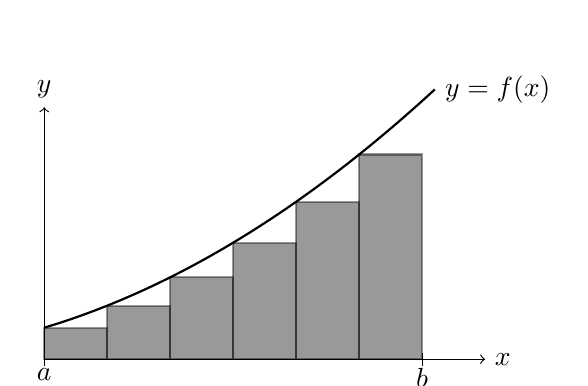
\begin{tikzpicture}[scale=0.8]
    \draw[->] (0,0) -- (7,0) node[right] {$x$};
    \draw[->] (0,0) -- (0,4) node[above] {$y$};

    \draw[domain=0:6.2, smooth, thick] plot (\x, {0.5+0.3*\x + 0.05*\x*\x}) node[right] {$y=f(x)$};

    \foreach \i in {0,...,5} {
        \pgfmathsetmacro{\x}{\i}
        \pgfmathsetmacro{\fx}{0.5+0.3*\x + 0.05*\x*\x}
        \draw[fill=black, draw=black, thick, opacity=.4] (\x,0) rectangle (\x+1,\fx);
    }

    \draw (0,-0.1) -- (0,0.1) node[below=2pt] {$a$};
    \draw (6,-0.1) -- (6,0.1) node[below=2pt] {$b$};
\end{tikzpicture}
\end{center}
\subsection{Definition of Riemann Sum}
Let $f(x)$ be defined on a closed interval $[a, b]$, and let $a = x_0 < x_1 < \cdots < x_n = b$ be a partition of the interval. For each subinterval $[x_{i-1}, x_i]$, define:
\[
    \Delta x_i = x_i - x_{i-1}, \quad c_i \in [x_{i-1}, x_i]
\]
Then the sum
\[
    \sum_{i=1}^n f(c_i) \Delta x_i
\]
is called a \textbf{Riemann sum} of $f$ over $[a, b]$.
\subsection{Definition of a Definite Integral}
If the limit of the Riemann sums exists as the maximum subinterval width approaches zero:
\[
    \max \Delta x_i \to 0
\]
and gives the same value regardless of how the sample points $c_i$ are chosen, then the function $f$ is said to be integrable on $[a, b]$, and the \textbf{definite integral} is defined by:
\[
    \int_a^b f(x)\, dx = \lim_{\max \Delta x_i \to 0} \sum_{i=1}^n f(c_i) \Delta x_i
\]
\begin{center}
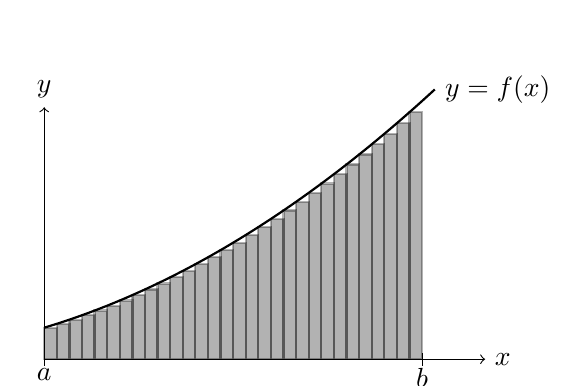
\begin{tikzpicture}[scale=0.8]
    \draw[->] (0,0) -- (7,0) node[right] {$x$};
    \draw[->] (0,0) -- (0,4) node[above] {$y$};

    \draw[domain=0:6.2, smooth, thick] plot (\x, {0.5 + 0.3*\x + 0.05*\x*\x}) node[right] {$y=f(x)$};

    \foreach \i in {0,...,29} {
        \pgfmathsetmacro{\x}{0.2*\i}
        \pgfmathsetmacro{\fx}{0.5 + 0.3*\x + 0.05*\x*\x}
        \draw[fill=black, draw=black, thick, opacity=.3] (\x,0) rectangle ({\x+0.2}, \fx);
    }

    \draw (0,-0.1) -- (0,0.1) node[below=2pt] {$a$};
    \draw (6,-0.1) -- (6,0.1) node[below=2pt] {$b$};
\end{tikzpicture}
\end{center}
Thus, the definite integral $\displaystyle\int_a^b f(x)\, dx$ represents the exact area under the curve $y = f(x)$ from $a$ to $b$, as the number of rectangles increases and their width approaches zero.
\subsection{Property of Definite Integrals}
\begin{enumerate}
    \item If $f$ is defined on $[a,b]$, and $\displaystyle\lim_{max \Delta x_i\to 0}\sum_{i=1}^{n}f(c_i)\Delta x_i$ exists, 
        then $f$ is integrable on $[a,b]$.
    \item If $f$ is continuous on $[a,b]$, then $f$ is integrable on $[a,b]$.
    \item If $f(x)$, $g(x)$, and $h(x)$ are integrable on $[a,b]$, then
    \begin{enumerate}
        \item $
            \displaystyle
            \int_a^af(x)\,dx =0
        $
        \item $
            \displaystyle
            \int_a^bf(x)\,dx =-\int_b^af(x)\,dx
        $
        \item $
            \displaystyle
            \int_a^bf(x)\,dx =-\int_b^af(x)\,dx
        $
        \item $
            \displaystyle
            \int_{-a}^af(x)\,dx =2\int_0^af(x)\,dx\text{, if $f(x)$ is even}
        $
        \item $
            \displaystyle
            \int_{-a}^af(x)\,dx =0\text{, if $f(x)$ is odd}
        $
        \item $
            \displaystyle
            \left|\int_a^bf(x)\,dx\right|\leq\int_a^b|f(x)|\,dx
        $
        \item $
            \displaystyle
            \int_a^bg(x)\,dx\leq\int_a^bf(x)\,dx\leq\int_a^bh(x)\,dx \text{, provided that } g(x)\leq f(x)\leq h(x)\text{ on }[a,b]
        $
        \item $
            \displaystyle
            \int_a^cf(x)\,dx=\int_a^bf(x)\,dx+\int_b^cf(x)\,dx
        $
    \end{enumerate}
\end{enumerate}
\section{Fundamental Theorems of Calculus}
\subsection{First Fundamental Theorem of Calculus}
If $f$ is continuous on $[a,b]$ and $\displaystyle F(x)=\int_a^xf(t)\,dt$, 
then $F'(x)=f(x)$ at every point $x$ in $[a,b]$
\subsection{Second Fundamental Theorem of Calculus}
If $f$ is continuous on $[a,b]$ and $F$ is an antiderivative of $f$, then
\[
    \int_a^bf(x)\,dx=\left.F(x)\right|_a^b=F(b)-F(a)
\]
Thus,
\[
    \boxed{
        \frac{d}{dx}\int_{v(x)}^{u(x)}f(t)\,dt=f(u(x))\cdot u'(x) - f(v(x)) \cdot v'(x)
    }
\]
\section{Integration Techniques}
\subsection{U-Substitution}
The \textbf{u-substitution method} is used to evaluate integrals by making a change of variables. 
If an integral contains a composite function, we can simplify it using a substitution.\\
Let $u = g(x)$, then:
\[
    \frac{du}{dx} = g'(x) \quad \Rightarrow \quad du = g'(x)\,dx
\]
So:
\[
    \int f(g(x))\,g'(x)\,dx \Rightarrow\int f(u)\,du
\]After integration, 
substitute back $u = g(x)$ to return to the original variable.
\subsubsection*{Example:}
Evaluate:
\[
    \int 2x\cos(x^2)\,dx
\]
Let
\[
    u=x^2\Rightarrow du=2xdx
\]
Thus
\[
    \begin{aligned}
        &\int 2x\cos(x^2)\,dx\\
        &= \int \cos(u)\,dx\\
        &= \sin(u)\\
        &= \sin(x^2)
    \end{aligned}
\]
\subsection{Trigonometric Substitution}
Trigonometric substitution is a technique used to evaluate integrals involving square roots of quadratic expressions. The key idea is to use a trigonometric identity to simplify the integrand.
Consider using trigonometric substitution when integrand contains expressions of the form:
\begin{itemize}
    \item $\sqrt{a^2 - x^2}$ — use $x = a \sin x$
    \item $\sqrt{a^2 + x^2}$ — use $x = a \tan x$
    \item $\sqrt{x^2 - a^2}$ — use $x = a \sec x$
\end{itemize}\textbf{Trigonometric Identities Used}
\begin{itemize}
    \item $\sin^2 x + \cos^2 x = 1$
    \item $\tan^2 x + 1 = \sec^2 x$
\end{itemize}
\subsubsection*{Example:}
Evaluate:
\[
    \int \frac{dx}{\sqrt{a^2-x^2}}
\]
Let
\[
    x=a\sin\theta \Rightarrow dx=\cos\theta\,d\theta
\]
And
\[
    \sqrt{a^2-x^2}=\cos\theta
\]
Thus
\[
    \begin{aligned}
        &\int \frac{dx}{\sqrt{a^2-x^2}}\\[.5em]
        &=\int\,d\theta\\[.5em]
        &=\theta\\[.5em]
        &=\arcsin(\frac{x}{a})+C
    \end{aligned}
\]
\subsection{Partial Fraction Decomposition}
Partial fraction decomposition is a method used to break a rational function into simpler fractions that are easier to integrate.
Given a rational function:
\[
    \frac{P(x)}{Q(x)} \quad \text{where } \deg P(x) < \deg Q(x),
\]
we can express it as a sum of simpler rational expressions depending on the factorization of $Q(x)$.\\[.5em]
\textbf{Types of Decompositions}\\[.5em]
\noindent
Let $Q(x)$ be factored as:
\[
    Q(x) = (x - r_1)^{k_1}(x - r_2)^{k_2}\cdots (x^2 + bx + c)^m\cdots
\]Then:
\begin{itemize}
    \item For each distinct linear factor $(x - r)^k$, include terms:
    \[
    \frac{A_1}{x - r} + \frac{A_2}{(x - r)^2} + \cdots + \frac{A_k}{(x - r)^k}
    \]
    
    \item For each irreducible quadratic factor $(x^2 + bx + c)^m$, include:
    \[
    \frac{Bx + C}{x^2 + bx + c} + \frac{Dx + E}{(x^2 + bx + c)^2} + \cdots + \frac{Yx + Z}{(x^2 + bx + c)^m}
    \]
\end{itemize}
\noindent
\textbf{Process}
\begin{enumerate}
    \item If improper ($\deg P(x) \geq \deg Q(x)$), perform long division first.
    \item Factor the denominator $Q(x)$.
    \item Set up partial fractions based on the types above.
    \item Multiply both sides by $Q(x)$ to eliminate denominators.
    \item Solve for constants by plugging in values or equating coefficients.
    \item Integrate each term individually.
\end{enumerate}
\subsubsection*{Example:}
Evaluate:
\[
    \int \frac{5x+7}{(x-1)(x+2)}\,dx
\]
Decompose
\[
    \frac{5x+7}{(x-1)(x+2)}=\frac{A}{(x-1)}+\frac{B}{(x+2)}
\]
Match coefficients
\[
    A+B=5, 2A-B=7\Rightarrow A=4\,,B=1
\]
Thus
\[
    \begin{aligned}
        &\int \frac{5x+7}{(x-1)(x+2)}\,dx\\[.5em]
        &=\int\left(\frac{4}{(x-1)}+\frac{1}{(x+2)}\right)\,dx\\[.5em]
        &=4\ln|x-1|+\ln|x+2|+C
    \end{aligned}
\]
\subsection{Integration by Parts}
\textbf{Integration by parts} is based on the product \textbf{rule for differentiation} and is given by:
\[
  \boxed{
    \int u \, dv = uv - \int v \, du
  }
\]
Where:
\begin{itemize}
    \item $u = \text{part to differentiate (becomes } du)$
    \item $dv = \text{part to integrate (becomes } v)$
\end{itemize}\textbf{Mnemonic: LIATE Rule}\\
\noindent Choose $u$ based on the following priority:
\begin{enumerate}
    \item \textbf{L}ogarithmic (e.g., $\ln x$)
    \item \textbf{I}nverse trig (e.g., $\tan^{-1} x$)
    \item \textbf{A}lgebraic (e.g., $x^2$)
    \item \textbf{T}rigonometric (e.g., $\sin x$)
    \item \textbf{E}xponential (e.g., $e^x$)
\end{enumerate}
\subsubsection*{Example:}
Evaluate:
\[
    \int xe^x\,dx
\]
LIATE: 
\[
    \begin{aligned}
        &u=x,\,dv=e^x\\
        \Rightarrow\, &du=dx,\,v=\int e^x\,dx=e^x
    \end{aligned}
\]
Thus
\[
    \begin{aligned}
        &\int xe^x\,dx\\[.5em]
        &=xe^x - \int e^x\,dx\\[.5em]
        &=xe^x - e^x\\[.5em]
        &=(x-1)e^x+C
    \end{aligned}
\]
\subsection{The DI Method}
This is a graph variation of Integration By Part
\begin{enumerate}
    \item Choose $f(x)$ to differentiate, and $g(x)$ to integrate.
    \item Alternate the signs starting with $+$.
    \item Multiply diagonally (Derivative term $\times$ Integral term just below) and alternate the signs.
    \item Stop the process when:
        \begin{itemize}
            \item The derivative reaches zero ($f^{(n)}(x) = 0$)
            \item Repeated derivatives cycle or become too complex
            \item Cyclic or repeating patterns
            \item The remaining integral is simpler to evaluate directly
        \end{itemize}
\end{enumerate}
\textbf{Final Expression:} Combine diagonals with alternating signs:
\begin{center}
        \renewcommand{\arraystretch}{2}
        \begin{tabular}{c|c|c}
            \textbf{Sign} & \textbf{Derivative(D)} & \textbf{Integral(I)} \\
            \hline
            $+$ \qquad& $f(x)$         \qquad& $ g(x) $ \\
            $-$ \qquad& $f'(x)$        \qquad& $\int g(x) \, dx$ \\
            $+$ \qquad& $f''(x)$       \qquad& $\iint g(x) \, dx$ \\
            $-$ \qquad& $f^{(3)}(x)$   \qquad& $\iiint g(x) \, dx$ \\
            $\vdots$ & $\vdots$ & $\vdots$ \\
        \end{tabular}
\end{center}
\[
    \int f(x) g(x) \, dx = f(x) \int g(x)\,dx - f'(x) \iint g(x)\,dx + \cdots
\]
\subsection{The King's Rule for Definite Integral}
King's Rule is a clever substitution technique in which we let $u=a+b-x$, and thus
\[
    \boxed{
        \int_a^b f(x)\,dx = \int_a^b f(a + b - x)\,dx
    }
\]By averaging both expressions:
\[
    \int_a^b f(x)\,dx = \frac{1}{2} \int_a^b \left[ f(x) + f(a + b - x) \right] dx
\]This is useful when $f(x) + f(a + b - x)$ is a constant or simplifies significantly.
\subsubsection*{Example:}
Evaluate:
\[
    I=\int_0^{\frac{\pi}{2}} \sin^2 x \,dx
\]
Apply the King's rule
\[
    I=\int_0^{\frac{\pi}{2}}\sin^2(\frac{\pi}{2}-x)\,dx=\int_0^{\frac{\pi}{2}}\cos^2 x\,dx
\]
Thus
\[
    \begin{aligned}
        2I&=\int_0^{\frac{\pi}{2}} \sin^2 x \,dx+\int_0^{\frac{\pi}{2}}\cos^2 x\,dx\\[.5em]
        &=\int_0^{\frac{\pi}{2}}\left(\sin^2 x + \cos^2 x\right)\,dx\\[.5em]
        &=\int_0^{\frac{\pi}{2}}1\,dx\\[.5em]
        &=\frac{\pi}{2}\\[.5em]
        I&=\frac{1}{2}\cdot\frac{\pi}{2}=\frac{\pi}{4}
    \end{aligned}
\]
\subsection{Feynman's Integration Technique for Definite Integral}
\textbf{Leibniz Integral Rule, or Differentiation under the Integral Sign} is a powerful technique used to evaluate integrals that depend on a parameter. This method became widely known through physicist Richard Feynman, who used it extensively in both theoretical and applied contexts.
It allows us to compute an integral by introducing a parameter, differentiating with respect to that parameter under the integral sign, simplifying the expression, and then integrating the result.\\[.5em]
\textbf{Leibniz Integral Rule}
\[
    \frac{d}{dx} \int_{u(x)}^{v(x)} f(x, t) \, dt
    = f(v(x), t) \cdot \frac{dv}{dx} - f(u(x), t) \cdot \frac{du}{dx} 
    + \int_{u(x)}^{v(x)} \frac{\partial f}{\partial x}(x, t) \, dt
\]\\[.5em]
If we take $u(x)$ and $v(x)$ as constants $a$ and $b$, then:
\[
    \boxed{
        \frac{d}{dx} \int_a^b f(x, t) \, dt = \int_a^b \frac{\partial f}{\partial x}(x, t) \, dt
    }
\]
\textbf{Conditions for Validity}\\
To apply this technique, we generally require:
\begin{itemize}
    \item $f(x, t)$ and $\partial f / \partial x$ are continuous in a region around the domain of integration.
    \item The limits $u(x), v(x)$ are differentiable functions of $x$.
    \item The integral $I(x)$ converges.
\end{itemize}
\textbf{Introducing a Parameter $\alpha$ to Simplify a Complex Integral}\\
One of the most clever applications of this technique is to evaluate a complicated integral by introducing a parameter \(\alpha\) that does not initially exist in the original integral. The idea is to construct a new, easier-to-handle integral:
\[
    I(\alpha) = \int_{a}^{b} f(x, \alpha) \, dx
\]
such that:
\begin{itemize}
    \item The original integral is recovered by evaluating $I(\alpha)$ at some specific value of \(\alpha\).
    \item Differentiating with respect to $\alpha$ simplifies the integrand.
\end{itemize}
\textbf{Steps:}
\begin{enumerate}
    \item Embed the difficult integral into a parameterized family $I(\alpha)$.
    \item Compute $\displaystyle\frac{dI}{d\alpha}$ under the integral sign.
    \item Integrate $\displaystyle\frac{dI}{d\alpha}$ with respect to $\alpha$ to recover $I(\alpha)$.
    \item Evaluate $I(\alpha)$ at the desired value (e.g., $\alpha = 0$) to obtain the original result.
\end{enumerate}
\subsubsection*{Example 1}
Evaluate:
\[
    \int_0^1 \frac{x^2-1}{\ln x}\,dx
\]
\textbf{Step 1: }Parameterize the Integrand\\
Let
\[
    I(\alpha)=\int_0^1 \frac{x^\alpha-1}{\ln x}\,dx
\]Note that:
\[
    I(0)=\int_0^1 \frac{x^0-1}{\ln x}\,dx=0\text{, and }I(2)\text{ is the original integral}
\]
\textbf{Step 2: }Now we compute
\[
    \begin{split}
        \frac{d}{d\alpha}I(\alpha)&=\int_0^1 \frac{\partial}{\partial\alpha}\frac{x^\alpha-1}{\ln x}\,dx=\int_0^1 x^\alpha dx\\
        &=\left.\frac{1}{\alpha +1}x^{\alpha +1}\right|_0^1\\
        &=\frac{1}{\alpha + 1} 
    \end{split}
\]
\textbf{Step 3: }Recover $I(\alpha)$
\[
    \begin{split}
        I(\alpha)&=\int \frac{d}{d\alpha}I(\alpha)\,d\alpha\\
        &=\int \frac{1}{\alpha + 1}\,d\alpha\\
        &=\ln(\alpha + 1)+C
    \end{split}
\]Recall $I(0)=0 \Rightarrow C=0$. So:
\[
    0=\ln(\alpha + 1)+C\Rightarrow C=0
\]
Hence:
\[
    I(\alpha)=\ln(\alpha + 1)
\]
\textbf{Step 4: }Evaluate $I(\alpha)$ at $\alpha = 2$
\[
    I(2)=\ln(2 + 1)=\ln3
\]
\textbf{Answer: }
\[
    \int_0^1 \frac{x^2-1}{\ln x}\,dx=\ln3
\]
\subsubsection*{Example 2}
Evaluate:
\[
    \int_0^{\infty} \frac{\sin x}{x}\,dx
\]
\textbf{Step 1: }Introduce an auxiliary exponential factor\\
Let
\[
    I(\alpha) = \int_0^{\infty} e^{-\alpha x} \frac{\sin x}{x} \, dx, \quad \alpha > 0
\]
\textbf{Step 2: }Now we compute
\[
    \frac{dI}{d\alpha} = -\int_0^{\infty} e^{-\alpha x} \sin x \, dx
\]
This integral is elementary:
\[
    \int_0^{\infty} e^{-\alpha x} \sin x \, dx = \frac{1}{1 + \alpha^2}
    \Rightarrow \frac{dI}{d\alpha} = -\frac{1}{1 + \alpha^2}
\]
\textbf{Step 3: }Recover $I(\alpha)$
\[
    I(\alpha) = -\int \frac{1}{1 + \alpha^2} \, d\alpha = -\tan^{-1}(\alpha) + C
\]
As $\alpha \to \infty$, $I(\alpha) \to 0$. So:
\[
    0 = -\tan^{-1}(\infty) + C = -\frac{\pi}{2} + C \Rightarrow C = \frac{\pi}{2}
\]
Hence:
\[
    I(\alpha) = - \tan^{-1}(\alpha)+\frac{\pi}{2}
\]
\textbf{Step 4: }Evaluate $I(\alpha)$ as $\alpha \to 0$
\[
    \lim_{\alpha \to 0} I(\alpha) = -\tan^{-1}(0)+\frac{\pi}{2} = \frac{\pi}{2}
\]
\textbf{Answer: }
\[
    \int_0^{\infty} \frac{\sin x}{x}\,dx=\frac{\pi}{2}
\]

\section{Improper Integral}
In some cases, definite integrals involve infinite intervals or integrands that become unbounded. Such integrals are called \textbf{improper integrals}. We define these using limits.
\subsection{Infinite Interval of Integration}
Let $f(x)$ be a function defined on $[a, \infty)$. Then the improper integral of $f$ from $a$ to $\infty$ is defined as:
\[
    \int_a^{\infty} f(x)\,dx := \lim_{b \to \infty} \int_a^b f(x)\,dx
\]
Similarly, if $f$ is defined on $(-\infty, b]$, we define:
\[
    \int_{-\infty}^{b} f(x)\,dx := \lim_{a \to -\infty} \int_a^b f(x)\,dx
\]
If $f$ is defined on $(-\infty, \infty)$, then:
\[
    \int_{-\infty}^{\infty} f(x)\,dx := \lim_{a \to -\infty} \int_a^c f(x)\,dx + \lim_{b \to \infty} \int_c^b f(x)\,dx
\]
for some finite number $c \in \mathbb{R}$.\\[.5em]
\textit{Note: Both limits must exist and be finite for the integral to converge.}
\subsection{Discontinuous Integrand}
Suppose $f$ is continuous on $(a, b]$ but has an infinite discontinuity at $a$. Then:
\[
    \int_a^b f(x)\,dx := \lim_{\epsilon \to a^+} \int_{\epsilon}^b f(x)\,dx
\]
Similarly, if $f$ has an infinite discontinuity at $b$, then:
\[
    \int_a^b f(x)\,dx := \lim_{\epsilon \to b^-} \int_a^{\epsilon} f(x)\,dx
\]
If the discontinuity is at an interior point $c \in (a,b)$, split the integral:
\[
    \int_a^b f(x)\,dx := \lim_{\epsilon \to c^-} \int_a^{\epsilon} f(x)\,dx + \lim_{\delta \to c^+} \int_{\delta}^b f(x)\,dx
\]
Each part must be interpreted as a limit, and the total integral converges if both one-sided integrals converge.
\subsection{Absolute vs Conditional Convergence}
\begin{itemize}
    \item If $\displaystyle\int_a^{\infty} |f(x)|\,dx$ converges, then $\displaystyle\int_a^{\infty} f(x)\,dx$ is said to be \textbf{absolutely convergent}.
    \item If $\displaystyle\int_a^{\infty} f(x)\,dx$ converges but $\displaystyle\int_a^{\infty} |f(x)|\,dx$ diverges, it is \textbf{conditionally convergent}.
\end{itemize}
\section{Application}
\subsection{Area}
\subsubsection{Approximating the Area Under the Curve}
\subsubsection*{Rectangular Approximation}
The area under the curve using $n$ rectangles of equal length is approximately:
\[
    \sum_{i=1}^n\text{(area of rectangle)}=
    \begin{cases}
        \,\displaystyle\sum_{i=1}^nf(x_{i-1})\Delta x\text{ left-endpoint rectangles}\\[15pt]
        \,\displaystyle\sum_{i=1}^nf(x_i)\Delta x\text{ right-endpoint rectangles}\\[15pt]
        \,\displaystyle\sum_{i=1}^nf(\frac{x_i+x_{i+1}}{2})\Delta x\text{ midpoint rectangles}
    \end{cases}
\]where $\displaystyle\Delta x=\frac{b-a}{n}$ and $a=x_0<x_1<x_2<\dots<x_n=b$
\begin{figure}[H]
    \centering
    \begin{minipage}{0.32\textwidth}
        \centering
        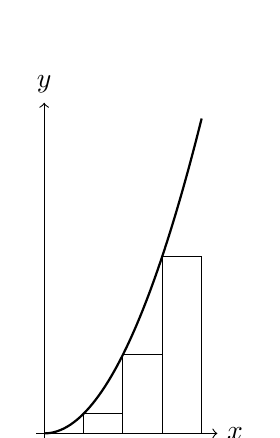
\begin{tikzpicture}[scale=1]
            \draw[->] (-0.1,0) -- (2.2,0) node[right] {$x$};
            \draw[->] (0,-0.1) -- (0,4.2) node[above] {$y$};
            \foreach \i in {0,...,3} {
                \pgfmathsetmacro{\xleft}{\i*0.5}
                \pgfmathsetmacro{\height}{\xleft*\xleft}
                \draw[black] (\xleft,0) rectangle ({\xleft+0.5}, {\height});
            }
            \draw[domain=0:2, smooth, variable=\x, thick] plot ({\x}, {\x*\x});
        \end{tikzpicture}
        \caption*{Left Endpoint}
    \end{minipage}
    \hfill
    \begin{minipage}{0.32\textwidth}
        \centering
        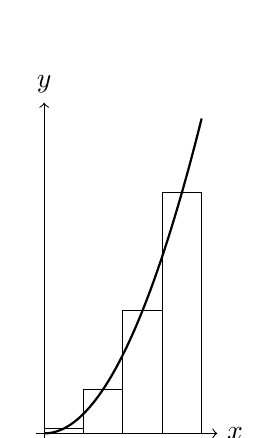
\begin{tikzpicture}[scale=1]
            \draw[->] (-0.1,0) -- (2.2,0) node[right] {$x$};
            \draw[->] (0,-0.1) -- (0,4.2) node[above] {$y$};
            \foreach \i in {0,...,3} {
                \pgfmathsetmacro{\xleft}{\i*0.5}
                \pgfmathsetmacro{\xmid}{\xleft + 0.25}
                \pgfmathsetmacro{\height}{\xmid*\xmid}
                \draw[black] (\xleft,0) rectangle ({\xleft+0.5}, {\height});
            }
            \draw[domain=0:2, smooth, variable=\x, thick] plot ({\x}, {\x*\x});
        \end{tikzpicture}
        \caption*{Midpoint}
    \end{minipage}
    \hfill
    \begin{minipage}{0.32\textwidth}
        \centering
        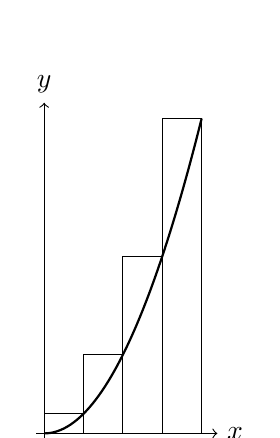
\begin{tikzpicture}[scale=1]
            \draw[->] (-0.1,0) -- (2.2,0) node[right] {$x$};
            \draw[->] (0,-0.1) -- (0,4.2) node[above] {$y$};
            \foreach \i in {0,...,3} {
                \pgfmathsetmacro{\xleft}{\i*0.5}
                \pgfmathsetmacro{\xright}{\xleft + 0.5}
                \pgfmathsetmacro{\height}{\xright*\xright}
                \draw[black] (\xleft,0) rectangle ({\xleft+0.5}, {\height});
            }
            \draw[domain=0:2, smooth, variable=\x, thick] plot ({\x}, {\x*\x});
        \end{tikzpicture}
        \caption*{Right Endpoint}
    \end{minipage}
\end{figure}
\subsubsection*{Trapezoidal Approximation}
\begin{figure}[H]
    \centering
    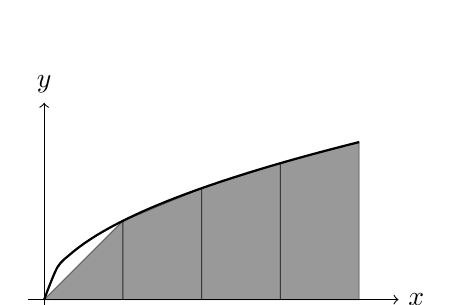
\begin{tikzpicture}[scale=1]
        \draw[->] (-0.2,0) -- (4.5,0) node[right] {$x$};
        \draw[->] (0,-0.2) -- (0,2.5) node[above] {$y$};
        \foreach \i in {0,...,3} {
            \pgfmathsetmacro{\xleft}{\i}
            \pgfmathsetmacro{\xright}{\xleft + 1}
            \pgfmathsetmacro{\yleft}{sqrt(\xleft)}
            \pgfmathsetmacro{\yright}{sqrt(\xright)}
            \draw[draw=black, fill=black, opacity=.4]
                (\xleft,0) -- (\xleft,\yleft) -- (\xright,\yright) -- (\xright,0) -- cycle;
        }
        \draw[domain=0:4, smooth, variable=\x, thick] plot ({\x}, {sqrt(\x)});
    \end{tikzpicture}
\end{figure}
If $f$ is continuous, the area under the curve of $f$ from $x=a$ to $x=b$ is:
\[
    \displaystyle
    \text{Area} \simeq\frac{b-a}{2n}\left[f(x_0)+2f(x_1)+\dots+2f(x_{n-1})+f(x_n)\right]
\]
\subsubsection{Area Under a Curve}
\begin{figure}[H]
    \centering
    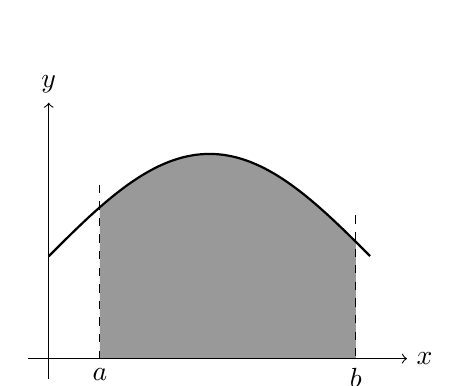
\begin{tikzpicture}[scale=1.3]
        \draw[->] (-0.2, 0) -- (3.5, 0) node[right] {$x$};
        \draw[->] (0, -0.2) -- (0, 2.5) node[above] {$y$};
        \draw[dashed] (.5,1.7) -- (.5,0) node[below]{$a$};
        \draw[dashed] (3,1.4) -- (3,0) node[below]{$b$};
        \begin{scope}
            \clip (.5,0) -- plot[domain=.5:3, smooth] (\x,{sin(\x r)+1}) -- (3,0) -- cycle;
            \fill[fill=black, opacity=.4] (0,0) rectangle (3.14,3);
        \end{scope}
        \draw[thick, black, domain=0:3.14, smooth, variable=\x] plot (\x,{sin(\x r)+1});
    \end{tikzpicture}
\end{figure}
The area under the graph of a continuous function $f(x)$ over the interval $[a, b]$ is given by the definite integral:
\[
    A = \int_a^b f(x)\,dx
\]
\noindent If $f(x) \geq 0$ on $[a, b]$, this integral gives the area between the curve and the $x$-axis. 
If $f(x)$ takes negative values, the integral represents \textbf{signed area}.
\subsubsection{Area Between Two Curves}
\begin{figure}[H]
    \centering
    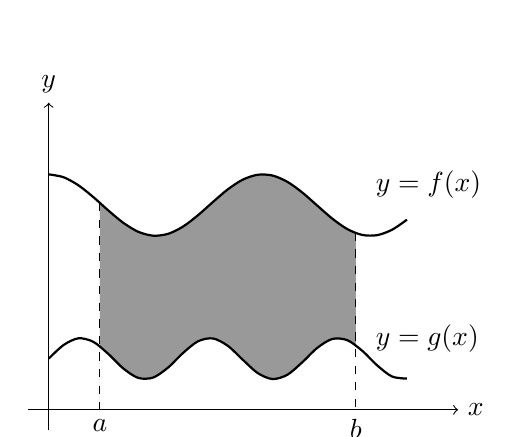
\begin{tikzpicture}[scale=1.3]
        \draw[->] (-0.2, 0) -- (4, 0) node[right] {$x$};
        \draw[->] (0, -0.2) -- (0, 3) node[above] {$y$};
        \draw[dashed] (.5,2.02) -- (.5,0) node[below]{$a$};
        \draw[dashed] (3,1.73) -- (3,0) node[below]{$b$};
        
        \begin{scope}
            \clip (.5,0) -- plot[domain=.5:3, smooth] (\x,{2 + 0.3*cos(3*\x r)}) -- plot[domain=3:.5, smooth] (\x,{0.5 + 0.2*sin(5*\x r)}) -- cycle;
            \fill[black, opacity=0.4] (0,0) rectangle (3.5,3);
        \end{scope}

        \draw[thick, domain=0:3.5, smooth, variable=\x] plot (\x,{2 + 0.3*cos(3*\x r)});
        \node[right] at (3.1, 2.2) {$y = f(x)$};

        \draw[thick, domain=0:3.5, smooth, variable=\x] plot (\x,{0.5 + 0.2*sin(5*\x r)});
        \node[right] at (3.1, 0.7) {$y = g(x)$};
    \end{tikzpicture}
\end{figure}
The area between two continuous functions \( f(x) \) and \( g(x) \) over the interval \([a, b]\), where \( f(x) \geq g(x) \), is given by:
\[
    A = \int_a^b \left[ f(x) - g(x) \right]\,dx
\]
This integral computes the net vertical distance between the top curve \( f(x) \) and the bottom curve \( g(x) \) at each point \( x \), accumulating the total area between them. It is essential that the functions be continuous on \([a, b]\) and that \( f(x) \geq g(x) \) holds throughout this interval to interpret the result as a positive area.
\subsection{Volumn}
\subsubsection{Cross Section}
\subsubsection{Disk Method}
\subsubsection{Washer Method}
\subsubsection{Shell Method}
\subsection{Arc Length and Surface Area}
\subsubsection{Arc Length}
Let $y = f(x)$ be a smooth curve on the interval $[a, b]$, where $f$ is differentiable and $f'(x)$ is continuous. The length of the curve from $x = a$ to $x = b$ is given by the arc length formula:
\[
    L = \int_a^b \sqrt{1 + \left(\frac{dy}{dx}\right)^2} \, dx
\]
\subsubsection{Surface Area}
Let $y = f(x)$ be continuous and differentiable on $[a, b]$, and suppose we rotate it about the $x$-axis. Then the surface area of the resulting solid is:
\[
    S = 2\pi y \int_a^b \sqrt{1 + \left(\frac{dy}{dx}\right)^2} \, dx
\]
\subsection{Average Value of a Function}
The average value of a continuous function $f(x)$ over the interval $[a, b]$ is given by:
\[
    f_{\text{avg}} = \frac{1}{b - a} \int_a^b f(x)\,dx
\]
\begin{figure}[H]
    \centering
    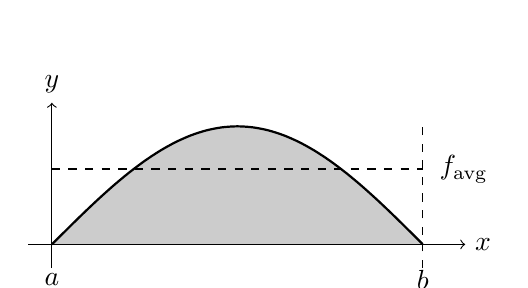
\begin{tikzpicture}[scale=1.5]
        \draw[->] (-0.2, 0) -- (3.5, 0) node[right] {$x$};
        \draw[->] (0, -0.2) -- (0, 1.2) node[above] {$y$};

        \draw[thick, domain=0:3.14, smooth, variable=\x] plot (\x,{sin(\x r)});

        \draw[dashed] (0,0) -- (0,1);
        \draw[dashed] (3.14,-.2) -- (3.14,1);
        \node at (0,-0.3) {$a$};
        \node at (3.14,-0.3) {$b$};

        \draw[dashed, thick] (0,0.6366) -- (3.14,0.6366);
        \node at (3.2,0.6366) [right] {$f_{\text{avg}}$};

        \begin{scope}
            \clip (0,0) -- plot[domain=0:3.14, smooth] (\x,{sin(\x r)}) -- (3.14,0) -- cycle;
            \fill[black, opacity=0.2] (0,0) rectangle (3.14,1.1);
        \end{scope}
    \end{tikzpicture}
\end{figure}
\section{Integration for Parametric}
\section{Integration for Polar}

\end{document}